\documentclass[12pt,fleqn]{article}
\usepackage{qual_ppgmc}
\usepackage [brazil]{babel}
\usepackage[utf8]{inputenc}
\usepackage{natbib}
\usepackage{fancyhdr}
\usepackage{color}
\usepackage{wallpaper} 
\usepackage{titlesec}   %% Define space between paragraph e section
\usepackage{float} 	%% Use to fix Figure or Table: ex: \begin{table}[H]
\usepackage{multirow}
\usepackage{graphics}
\usepackage{subfig}

%%%%Don't edit this block. It reduces the spacing between the lines of the references
\let\OLDthebibliography\thebibliography
\renewcommand\thebibliography[1]{\OLDthebibliography{#1} 
\setlength{\parskip}{0pt}\setlength{\itemsep}{0pt plus 0.3ex}}

%%-----------------------------------------------EDIT-----------------------------------------------
\title{INDICADOR INDIRETO DE ROTAÇÃO EM AGLOMERADOS DE GALÁXIAS}
%%-----------------------------------------------EDIT----------------------------------------------
\author
    {\rm \begin{tabular}{l} 
    \textbf{Luenne Nailam Sousa Nascimento}$^{1}$ - {\textnormal luennenailam@gmail.com}\\%
    \textbf{André Luis Batista Ribeiro}$^{1}$ - {\textnormal albr@uesc.br}\\
    {\fontsize{11}{0}\selectfont $^{1}$Universidade Estadual de Santa Cruz, UESC, Brasil}
  \end{tabular}}
%%----------------------------------------------------------------------------------------------

\fancypagestyle{firspagetstyle}
{
	\lhead{}
	\fancyhead[C]{%
		
\includegraphics[width=0.9\linewidth]{logo}\\%
		{\scriptsize \fontfamily{phv}\fontseries{b}\selectfont \color[rgb]{0.45,0.45,0.45}
		Relatório de Pesquisa \\
		Exame de Qualificação\\
		PPGMC\\
	    }
	}
	\renewcommand{\headrulewidth}{0.0pt}
	\fancyfoot[C]{\footnotesize \parbox{15cm} {\centering  \fontsize{7.5}{0}\selectfont \it Relatório de Pesquisa – Exame de Qualificação, 
	Ilhéus, BA – 04 Setembro 2019}} % \ttfamil
	\rhead{}
}


\begin{document}
\maketitle

\thispagestyle{firspagetstyle}

\fancyhead[L]{\footnotesize{\fontsize{7.5}{0}\selectfont \it Relatório de Pesquisa -  Exame de Qualificação\\
	Programa de Pós-Graduação em Modelagem Computacional em Ciência e Tecnologia\\}}
\renewcommand{\headrulewidth}{0.0pt}
\fancyfoot[C]{\footnotesize \parbox{15cm} {\centering  \fontsize{7.5}{0}\selectfont \it Relatório de Pesquisa -  Exame de Qualificação, Programa de 
Pós-Graduação em Modelagem Computacional em Ciência e Tecnologia, Universidade Estadual de Santa Cruz, Campus Soane Nazaré de Andrade - Ilhéus, BA, Brasil}} % \ttfamil
\rhead{}

\begin{abstract}
Aglomerados de galáxias são as maiores estruturas gravitacionalmente ligadas do Universo e são
constituídos por algumas dezenas a milhares de galáxias.
Eles possuem propriedades como as funções de massa e de correlação espacial, além de sua
própria evolução, cujas parametrizações podem restringir o modelo cosmológico
atual.  Consequentemente, o cálculo preciso das massas de aglomerados é de extrema
importância. Existem diversas abordagens aplicadas ao cálculo de massa de
aglomerados, sendo o método mais empregado aquele que utiliza as velocidades das galáxias membro dos
aglomerados e assume o equilíbrio dinâmico através do Teorema do Virial. 
Este método, apesar de sua ampla aplicabilidade, não leva em conta a possível
rotação dos aglomerados. A rotação desses sistemas seria uma decorrência de um impulso angular inicial
que teria perdurado desde a sua formação.  A rotação poderia surgir também 
em consequência de fusões ou interações com aglomerados vizinhos.
Não levar em consideração a rotação de aglomerados pode introduzir um erro no cálculo de sua
massa. Neste trabalho propomos um método para identificar a componente rotacional dos
aglomerados. O método de detecção de rotação foi implementado em linguagem R, e aplicado a uma amostra de 20 aglomerados localizados no Universo Local, sendo que 12 deles
apresentaram sinal significativo de rotação.
\end{abstract}

%\keywords{\em{Palabra chave 1, Palabra chave 2, Palabra chave 3 (Defina até 5 palabras chaves) }}
\noindent{\textbf{\textit{Palavras-chave: }}{\em{Aglomerados de galáxias, Rotação, Testes estatísticos. }}
\newpage

\pagestyle{fancy}

\section{INTRODUÇÃO}
Aglomerados de galáxias são as maiores estruturas do Universo observável que podem
ter alcançado o estado de equilíbrio dinâmico. Eles são constituídos por algumas dezenas até
milhares de galáxias ligadas pela força gravitacional. Para que as galáxias se mantenham
próximas umas das outras por longas escalas de tempo é necessário que exista uma
considerável força gravitacional que impeça a sua dispersão no espaço. Isto significa que a
massa típica desses sistemas é muito grande (o catálogo de Abell, por exemplo, possui sistemas
com massa total por volta de $10^{14}$ a $10^{15}$ massas solares), o que torna o mapeamento de
aglomerados e a correta obtenção de suas propriedades observadas de grande importância
tanto para estudos referentes ao processo de formação de estruturas no Universo, como para
restringir o modelo cosmológico atual (Velásquez, 2007).

Ao longo do século XX muitos trabalhos foram voltados ao estudo de aglomerados e
permitiram a sua crescente caracterização como um sistema físico bastante particular. Dessa
maneira, propriedades como: a distribuição de posições e de velocidades em aglomerados,
perfis de densidade numérica – entendimento quanto à distribuição das galáxias em relação a
sua distância ao centro do aglomerado –, funções de luminosidade – quantificar a distribuição
luminosa – e de massa, puderam ser obtidas e utilizadas para descrever aglomerados
(Velásquez, 2007). Além de parâmetros dinâmicos e cinemáticos como: velocidade média
(adequado a estimativa de distâncias); dispersão de velocidades (compreensão do grau de
ligação gravitacional entre galáxias); massas (entender o grau de contribuição de densidade
referente a massa total do Universo); e a razão massa/luminosidade (utilizada como indicativo
da quantidade matéria escura e para estimar se a distribuição de luz segue a da matéria)
(Friaça et al., 2008).

As conclusões alcançadas por esses trabalhos sugerem que os aglomerados iniciaram o
seu processo de formação há aproximadamente 10 bilhões de anos, processo que se dá de
forma continuada até os dias de hoje. Estudos baseados na distribuição de velocidades de
galáxias nesses sistemas indicam que apenas uma fração deles (em torno de 60\%) pode ser
considerada em estado de equilíbrio dinâmico. Os demais constituem sistemas ainda em
formação ou perturbados por interações com outros aglomerados. O grande número de
sistemas fora do equilíbrio pode introduzir dificuldades na interpretação das propriedades
dinâmicas dos aglomerados (Friaça et al., 2008).

Portanto, o entendimento preciso dos graus de liberdade de aglomerados é de extrema
importância para que seja possível realizar inferências dinâmicas sobre esses sistemas. Um
dos aspectos menos estudados a respeito de aglomerados é a possibilidade de que eles tenham
algum grau de rotação. Não levar em consideração a rotação de aglomerados pode gerar um
erro nas suas estimativas de massa, o que afeta diretamente as restrições cosmológicas
fornecidas pela função de massa desses sistemas (Fang et al., 2008).


\section{AGLOMERADOS DE GALÁXIAS}
Aglomerados de galáxias são definidos basicamente por três componentes: galáxias,
meio intra-aglomerado e matéria escura. A maior parte da massa do aglomerado, cerca de
80\% do total, é composta de matéria escura (não-bariônica). Do restante, na forma bariônica
(feita de prótons e nêutrons), 15\% são compreendidos de gás intra-aglomerado (MIA) e apenas
5\% da massa de um aglomerado estão na forma de estrelas de galáxias.

A busca por compreender a formação e evolução dos aglomerados de galáxias é uma
das questões mais importantes da Astrofísica. No paradigma atual de formação das estruturas,
as galáxias e os aglomerados surgem a partir de halos escuros. O resfriamento desses halos
ocasiona a formação de estruturas condensadas, onde depois colapsariam os bárions, formando 
os sistemas astrofísicos conhecidos. Este cenário seria ainda hierárquico, com a formação dos 
aglomerados ocorrendo após a formação das
galáxias, aproximadamente em um desvio para o vermelho $z \approx 2$ 
(Velásquez, 2007).


\begin{figure}[!htbp] %h or !htbp
\vspace{-2pt}
\begin{center}
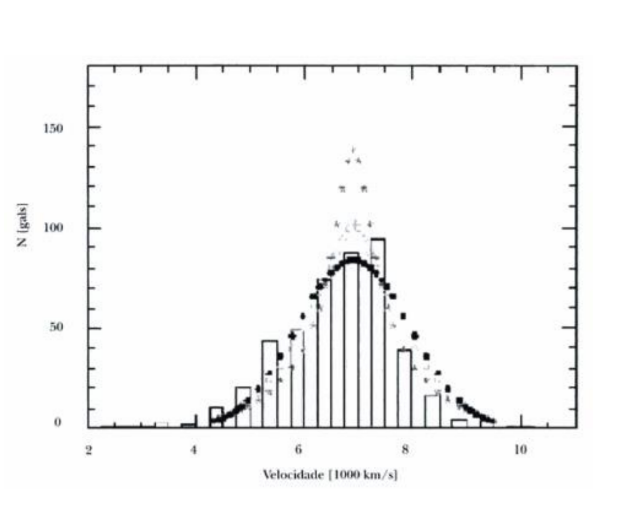
\includegraphics[height=6.7cm,width=9cm]{fig2}%
\caption{Histograma de velocidades no Aglomerado de Coma. Fonte:}
\label{fig1}%
\end{center}
\end{figure}


O processo de formação de aglomerados de galáxias ainda não atingiu o seu fim.
Enquanto regiões centrais estão em equilíbrio dinâmico, as regiões periféricas (externas)
acumulam matéria na forma de galáxias ou grupos de galáxias de modo contínuo. Comumente
o entorno dos aglomerados de galáxias é constituído de grupos de galáxias que podem ser
absorvidos pelo aglomerado principal ao longo do tempo, ocasionando o aumento de sua
massa (Rembold, 2011). Estudos sobre a distribuição de velocidades de galáxias em aglomerados indicam que a mesma possui distribuição Não Rejeita, vide Figura \ref{fig1}, ou muito bem ajustada por uma
gaussiana somente na região virializada do sistema (região mais interna do sistema) (Yahil \&
Vidal 1977), podendo existir sinais de múltiplos modos normais na região mais externa
(Ribeiro, Lopes \& Trevisan 2011), comprovando a presença de componentes de um sistema
em processo de evolução pelo acréscimo de matéria ao seu entorno. Esse
acréscimo de matéria, na forma de galáxias ou grupo de galáxias. 
Isto sugere que a formação de aglomerados de galáxias é
um processo contínuo que decorre de fusões sucessivas e encontros gravitacionais de maiores e menores proporções (Nascimento et al., 2016).



% \ \ \ \\newpage %
\subsection{Distribuição de Velocidades ao longo do Aglomerado}
A velocidade de uma galáxia contida em um aglomerado, em uma dada posição, não
pode ser maior que a velocidade de escape do sistema, caso isto aconteça a galáxia não
pertenceria mais ao aglomerado. A velocidade de escape e a distância ao centro do
aglomerado são grandezas inversamente proporcionais, ou seja, a velocidade de escape
decresce com o aumento da distância ao centro do aglomerado, portanto é mais fácil o escape
de uma galáxia que está na região periférica (de Oliveira e Viegas, 2004).

Para que o aglomerado exista como unidade dinâmica é preciso uma redução na amplitude da
distribuição de velocidades das galáxias à medida que haja um afastamento da região central.
O grande problema dessa propriedade é o efeito de projeção. As galáxias que estão com
distâncias distintas do centro do aglomerado podem parecer ao observador com mesma
distância em consequência da observação apenas das posições projetadas no plano do céu (de
Oliveira e Viegas, 2004).

Na Figura \ref{fig2} vemos a distribuição de velocidades do aglomerado de
 Coma (um dos mais estudados no Universo Local) em função da distância da
galáxia ao centro do aglomerado, onde o estreitamento da distribuição de velocidades
define uma espécie de "corneta" que pode ser utilizada para definir os membros
de um aglomerado, sendo removidas as galáxias que estejam
significativamente acima ou abaixo da "corneta".


\begin{figure}[!htbp] %h or !htbp
\vspace{-2pt}
\begin{center}
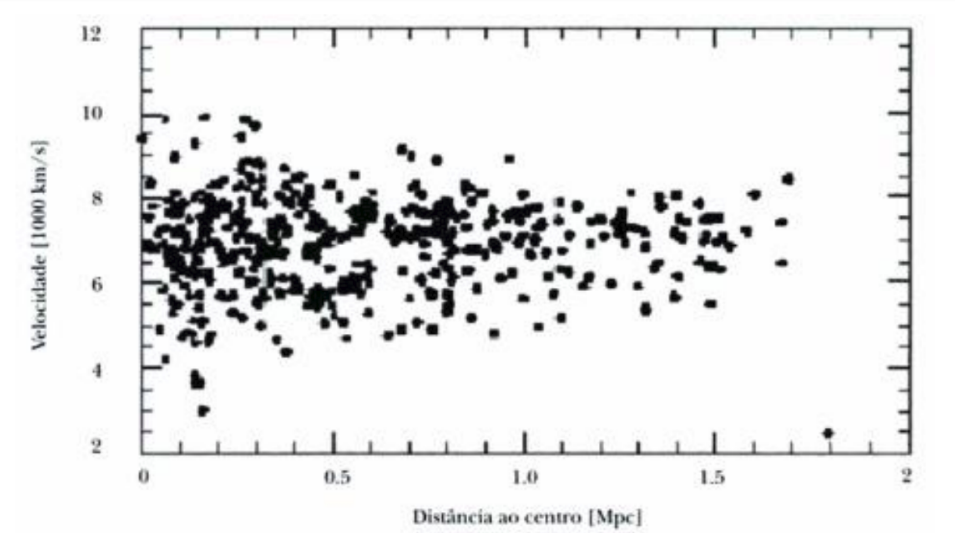
\includegraphics[height=6.7cm,width=9cm]{fig1}%
\caption{Distribuição de velocidades em função da distância ao centro do Aglomerado de Coma. Fonte:}
\label{fig2}%
\end{center}
\end{figure}

\subsection{Rotação de Aglomerados}
O conhecimento do estado dinâmico de aglomerados de galáxias pode propiciar restrições importantes em cenários cosmológicos, como a determinação da massa total do aglomerado e uma estimativa da quantidade de matéria escura no Universo. A possibilidade da existência de aglomerados em rotação tem sido discutida por muitos autores (por exemplo, veja os estudos de Hwang \& Lee 2007; Manaloupoulos \& Plionis 2016). 

Para detecção de indícios de rotação, Hwang \& Lee (2007) utilizaram dados espectroscópicos do \textit{Sloan Digital Sky Survey} \footnote{Considerado o mais ambicioso mapeamento astronômico que já foi feito. Com este mapeamento, os astrônomos podem observar os padrões de grande escala das galáxias: filamentos e vazios em grandes regiões angulares do Universo.}(SDSS) e \textit{Two-Degree-Field Galaxy Redshift Survey} (2dF-GRS). A rotação de aglomerados foi modelada como a rotação de galáxias membro e a rotação do gás intra-aglomerado. Eles levantaram inicialmente a hipótese de que a rotação se origina através de fusões de aglomerados. Um aspecto importante do método empregado por Hwang \& Lee (2007) é que os aglomerados com rotação devem exibir divisão espacial entre galáxias com velocidades maiores e menores que a velocidade média do aglomerado além de apresentar um pico no mapa de densidade. Nesta pesquisa de Hwang \& Lee (2007) foram detectados seis sistemas com rotação, em um total de dozes aglomerados (Abell 0954, Abell 1139, Abell 1399, Abell 2162, Abell 2169, and Abell 2366). Constatou-se ainda que estes aglomerados estão em equilíbrio dinâmico e não sofreram fusão recente, não dando suporte, portanto, à hipótese de interações como causadoras da rotação. 

Kalinkov et al. (2008) tentaram obter o gradiente máximo no campo de velocidades de Abell 2107 e determinaram que a direção do coeficiente de correlação linear máximo definiria o eixo maior do aglomerado e o eixo menor seria o de rotação. Foram utilizadas subamostras de galáxias membro, ordenadas de acordo a distância ao centro do aglomerado para definir o grau de rotação do sistema. Esse mesmo aglomerado foi estudado por Oegerle et al. (1992) e foram encontrados indícios de rotação. Materne et al. (1983) apontaram a dificuldade em diferenciar um aglomerado rotativo de dois que se sobrepõem, pelo motivo de estar se fundindo ou se afastando. Porém, o aglomerado  Abell 2107 não consiste de dois aglomerados sobrepostos, em consequência do pico estreito representado em seu histograma de velocidades. O indicador mais forte que definiu a rotação foi o ângulo de posição do eixo com o gradiente máximo no campo de velocidades quase coincidindo com o ângulo de posição do eixo com o maior alongamento.  Nesse estudo o período de rotação foi calculado em uma volta a cada $2.4\times10^9$ anos e houve uma correção no valor da massa para $2.8\times10^{14}~{\rm M_\odot}$  (a massa inicial era de $3.2\times10^{14}~{\rm M_\odot}$, sem levar em conta a rotação). 

Baseado no estudo da distribuição de velocidades das galáxias membro, Tovmassian (2015)  detectou
sinais de rotação em 17 de uma amostra de 65 aglomerados (26\%).
O método analisa o número de galáxias com velocidades mais baixas e mais altas que a velocidade média do aglomerado em diferentes partes do aglomerado. O método teve mais êxito em aglomerados planos, com $f=a/b > 1.8$ (a e b semieixos - maior e menor – da distribuição de galáxias do aglomerado). 
Para estes, a taxa de detecção de rotação foi mais alta (7 dos 18 aglomerados planos, 39\%).  Esse resultado suporta a opinião de que os aglomerados foram originalmente formados a partir das enormes nuvens de gás primordiais e preservaram a rotação das nuvens primordiais, a menos que sofram fusões com outros aglomerados e grupos de galáxias. 

Já na tese de Manolopoulou (2014) é realizado um estudo de um novo algoritmo para dedução de rotação usando a velocidade radial projetada\footnote{É a velocidade de um objeto na direção da linha de visada, isto é, a velocidade com que o objeto se aproxima ou se afasta do observador.}. Inicialmente os testes foram realizados em aglomerados gerados em simulações de Monte Carlo para confirmar se o método fornecia indicações robustas de rotação. Em seguida, aplicado em amostras de aglomerados de Abell. Através do teste de Kolmogorov-Smirnov, decidiu-se quanto a sua rotação significativa ou não, seu centro rotacional, orientação do eixo de rotação, amplitude de velocidade rotacional e, finalmente, o sentido de rotação no sentido horário ou anti-horário no plano do céu. Foram encontrados 23 aglomerados possivelmente rotativos dentro de 1.5 Mpc ou a uma distância de 2.5 Mpc do centro do aglomerado, do total de 45 da amostra.


\begin{figure}[!htbp] %h or !htbp
\vspace{-2pt}
\begin{center}
\includegraphics[height=9cm,width=9cm]{f7.pdf}%
\caption{Distribuição de galáxias no plano do céu do par de aglomerados A3407 e A3408. Fonte: Nascimento et al. 2016.}
\label{fig3}%
\end{center}
\end{figure}

Nascimento et al (2016), a partir de uma amostra de galáxias observadas no Cerro Tololo Interamerican Observatory (CTIO), realizaram um estudo dinâmico em torno do par de aglomerados de Abell (A3407 e A3408). O objetivo era verificar se a amostra correspondia a um simples sistema de galáxias ou a um processo de fusão, melhorando o entendimento desse sistema. Testes estatísticos foram aplicados aos membros mostrando que ambos os sistemas bem como cada aglomerado individual tem uma distribuição de velocidade Gaussiana. Um gradiente de velocidade de $\approx 847 \pm 114\; {\rm km~s^{-1}}$ foi identificada ao redor do eixo principal da distribuição de galáxias projetada indicando uma possível rotação. 
O estudo definiu um "gap" na distribuição de velocidades e realizou testes sobre a distribuição
espacial de galáxias (em torno do eixo principal do aglomerado) visando identificar diferenças
entre objetos com velocidades maiores e menores que a posição do "gap". Esta comparação
indicou que havia diferença significativa entre estas subamostras, sugerindo um grau de
rotação no sistema A3407+A3408 (vide Figura \ref{fig3}).

\section{METODOLOGIA}

O método proposto por Nascimento et al. (2016) para estudar um par de aglomerados
pode ser adaptado para o estudo da rotação de aglomerados individuais. Neste trabalho
fazemos esta adaptação e a implementamos em linguagem R. O código resultante
é aplicado a uma amostra
de 20 aglomerados ricos do SDSS, localizados em baixos $redshifts$, com espectroscopia
disponível para objetos com $m_r \leq 17.77$. Esta amostra foi estudada previamente
por Lopes et al. (2009) que definiu e selecionou as galáxias membro estatisticamente.
Em etapa posterior do trabalho, pretentemos analisar uma amostra com aproximadamente 500 
aglomerados do SDSS.

\subsection{Algoritmo}

A sequência de passos definidos por Nascimento et al. (2016) são:

\begin{enumerate}
\item  Estudar a distribuição de velocidades das galáxias membro do aglomerado
em busca de "gaps" significativos. A rotina visa identificar a probabilidade de que um "gap", 
de certo tamanho e em dada localização, possam ser produzidos a partir de amostragens
aleatórias retiradas de uma gaussiana. As velocidades das galáxias são ordenadas em ordem
crescent e o i-ésimo "gap" é definido como $g_i = v_{i+1} - v_i$. O "gap" é ponderado
pela sua posição, através de $w_i=i(N-i)$, onde $N$ é o número de galáxias do aglomerado.
Os "gaps" ponderados são Não Rejeitaizados através da divisão por meio da média (MM) da distribuição ordenada do "gap" ponderado dada por:

$$MM = \frac{2}{N} \sum_{i=N/4}^{3N/4} \sqrt{w_i g_i}$$

São buscados "gaps" com valores maiores que 2.25, uma vez que em retiradas aleatórias de
uma gaussian, "gaps" desse tamanho ocorrem no máximo em 3\% dos casos (vide Wainer \& Shacht 1978. Beers et al. 1991).

\item Em seguida os dados são divididos em duas amostras, contendo objetos
com velocidades maiores e velocidades menores que a do "gap", chamadas aqui
de amostras I e II.

\item Determina-se então o eixo principal do aglomerado como aquele resultante
do ajuste de uma elipse aos dados projetados no plano do céu. O ajuste é feito
usando-se o pacote {\bf ellipse} do R.

\item As amostras I e II são então comparadas em relação a sua distribuição 
de duas maneiras: independente do eixo principal e em cada lado do eixo.
Os testes de comparação de duas amostras utilizados foram o teste de Cramer 2D
e o de Hotelling. Uma revisão sobre testes estatísticos em geral, e uma
descrição específica destes dois testes são apresentadas no Apêndice
deste trabalho.

\item Dado que as distribuições espaciais das amostras  I e II sejam distintas
com 95\% de confiança em relação aos testes acima citados, interpretamos o resultado
como sendo uma indicação indireta de rotação nos aglomerados.

\item Para os aglomerados onde isto acontece, traçamos um perfil de velocidade
de rotação ao  longo da distância ao centro do aglomerado.

\item Caso o aglomerado não tenha "gap" significativo ($>$ 2.25), utilizamos a
mediana dos dados como divisor das velocidades do sistema.


\end{enumerate}

\newpage

\section{RESULTADOS PRELIMINARES}


Os resultados da aplicação de nosso método são apresentados
resumidamente nas Figuras 4 a 5 e nas tabelas 1 a 3. Na Figura 4, apresentamos
a análise de {\it gaps} para os 20 aglomerados da amostra. Cada gráfico na
figura contém o histograma da distribuição de velocidades, o ajuste gaussiano superposto,
barras inferiores indicando as velocidades individuais, sendo que em vermelho estão
indicados os {\it gaps} com valores maiores que 2.25, ou seja, os {\it gaps} significativos.
Quando mais de um {\it gap} é encontrado, escolhemos aquele de maior valor; finalmente,
a linha vertical tracejada indica a posição da BCG (brightest cluster galaxy) apenas
como referência. Na Figura 5, vemos o ajuste da elipse na distribuição (X,Y) projetada
no plano do céu, com os pontos acima ($+$) e abaixo ($-$) em relação à posição do \textit{gap} principal
 indicados em verde e rosa, respectivamente.
A posição da BCG é indicada com um losango vermelho.

A distribuição de galáxias em torno do {\it gap} de velocidades pode ser utilizada como um indicador indireto da presença ou não de rotação. Estudamos o quanto diferem espacialmente as galáxias de acordo com a sua posição em relação ao eixo principal. A hipótese nula dos testes é a de que os pontos $+$ e $-$ foram retirados da mesma população. Foram aplicados dois testes estatísticos, Cramer 2D e Hotelling, em três configurações diferentes: todos os pontos do gráfico, acima e abaixo do eixo principal (Tabelas \ref{table1}, \ref{table2}, \ref{table3}). O teste de Cramér para duas amostras pode ser usado para dados univariados e multivariados, 
como neste trabalho (vide Apêndice). Para o cálculo
do valor crítico uma rotina de {\it bootstrap} é utilizada, e métodos de permutação são usados para obter o valor-p do teste.
Neste trabalho usamos 1000 réplicas dos dados a cada caso. O teste de Hotelling multivariado compara médias em duas
amostras e também é descrito brevemente no Apêndice. A rejeição ou não da hipótese nula é feita em todos os casos
para um nível de 95\% de confiança. Nesta primeira aplicação do método, consideramos evidência significativa
de rotação se houve rejeição da hipótese nula em pelo menos uma das configurações testadas. Isto nos leva
a 12 aglomerados com evidência de algum grau de rotação. São eles os aglomerados: 02, 04, 05, 08, 09, 10, 11,
12, 14, 16, 17 e 18.

Finalmente, calculamos o perfil de velocidade de rotação do aglomerado para estes doze aglomerados, que são apresentados
na Figura \ref{fig6}. A velocidade de rotação foi calculada de maneira cumulativa contra o raio projetado das galáxias de acordo
com

\begin{equation}
\omega= \Delta V/R
\label{eq:eq10}
\end{equation}

\noindent onde $\Delta V$ é a diferença de velocidade entre os pontos $+$ e $-$ internos a $R$.


%\begin{table}[H] % !htbp 
%\caption{Teste Estatístico para comparação entre duas amostras em relação a \textit{p-value} para todos os pontos à direita do \textit{gap}.}
%\vspace{12pt}
%\centering{}
%\resizebox{.8\textwidth}{!}{
%\begin{tabular*}{\textwidth}{@{\extracolsep{\fill}}ccc}     
%\hline
%\textbf{Aglomerado} & \textbf{\textit{p-value}} &  \textbf{Diagnóstico} \\
%\hline
% 01 & 0.7767 & Não Rejeita \\  
%\hline
% 02 & 0.0089 &  Rejeita \\ 
%\hline
% 03 & 0.9024 & Não Rejeita \\ 
%\hline
% 04 & 0.0791 & Não Rejeita \\ 
%\hline
% 05 & 0.0507 & Não Rejeita \\ 
%\hline
% 06 & 0.3285 & Não Rejeita \\ 
%\hline
% 07 & 0.0543 & Não Rejeita \\ 
%\hline
% 08 & 0.7036 & Não Rejeita \\ 
%\hline
% 09 & 0.7157 & Não Rejeita \\ 
%\hline
% 10 & 0.5267 & Não Rejeita \\ 
%\hline
% 11 & 0.0656 & Não Rejeita \\ 
%\hline
% 12 & 0.9503 & Não Rejeita \\ 
%\hline
% 13 & 0.8944 & Não Rejeita \\ 
%\hline
% 14 & 0.0206 &  Rejeita \\ 
%\hline
% 15 & 0.9913 & Não Rejeita \\ 
%\hline
% 16 & 0.0020 &  Rejeita \\ 
%\hline
% 17 & 0.4376 & Não Rejeita \\ 
%\hline
% 18 & 0.0627 & Não Rejeita \\ 
%\hline
% 19 & 0.2143 & Não Rejeita \\ 
%\hline
% 20 &  0.7178 & Não Rejeita \\
%\hline
%\label{table1}
%\end{tabular*}
%}
%\end{table}


% TABLE EXAMPLE
%\begin{table}[H] % !htbp 
%\caption{Teste Estatístico para comparação entre duas amostras em relação a \textit{p-value} para todos os pontos à esquerda do \textit{gap}.}
%\vspace{12pt}
%\centering{}
%\resizebox{.8\textwidth}{!}{
%\begin{tabular*}{\textwidth}{@{\extracolsep{\fill}}ccc}     
%\hline
%\textbf{Aglomerado} & \textbf{\textit{p-value}} &  \textbf{Diagnóstico} \\
%\hline
%01 & 0.8775 & Não Rejeita \\  
%\hline
%02 & 0.1026 &  Rejeita \\ 
%\hline
%03 & 0.2907 & Não Rejeita \\ 
%\hline
%04 & 0.0002 &  Rejeita \\ 
%\hline
%05 & 0.5371 & Não Rejeita \\ 
%\hline
%06 & 0.5717 & Não Rejeita \\ 
%\hline
%07 & 0.3838 & Não Rejeita \\ 
%\hline
%08 & 0.1575 & Não Rejeita \\ 
%\hline
%09 & 0.3492 & Não Rejeita \\ 
%\hline
%10 & 0.5155 & Não Rejeita \\ 
%\hline
%11 &  0.2115 & Não Rejeita \\ 
%\hline
%12 &  0.0125 &  Rejeita \\ 
%\hline
%13 & 0.2035 & Não Rejeita \\ 
%\hline
%14 & 0.4879 & Não Rejeita \\ 
%\hline
%15 & 0.2061 & Não Rejeita \\ 
%\hline
%16 & 0.7035 & Não Rejeita \\ 
%\hline
%17 & 0.5239 & Não Rejeita \\ 
%\hline
%18 & 0.3018 & Não Rejeita \\ 
%\hline
%19 & 0.6839 & Não Rejeita \\ 
%\hline
%20 & 0.6321 & Não Rejeita \\
%\hline
%\label{table2}
%\end{tabular*}
%}
%\end{table}


\begin{figure}[H] %h or !htbp
\vspace{-2pt}
\centering
\subfloat{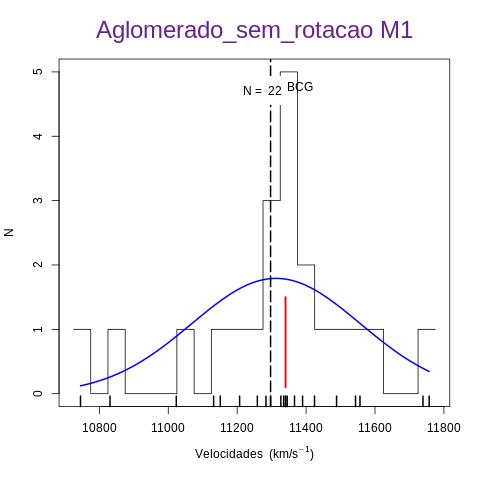
\includegraphics[scale=.23]{resultados/dist1}}
\subfloat{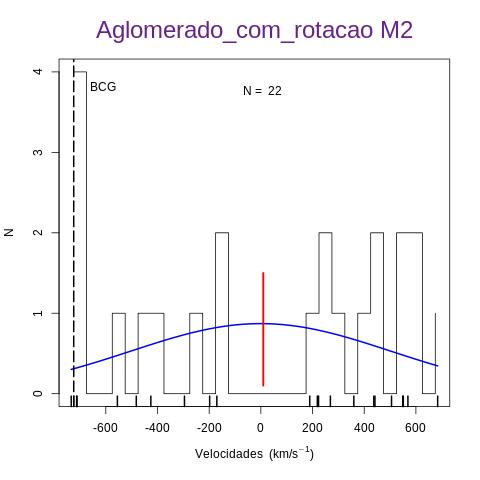
\includegraphics[scale=.23]{resultados/dist2}}
\subfloat{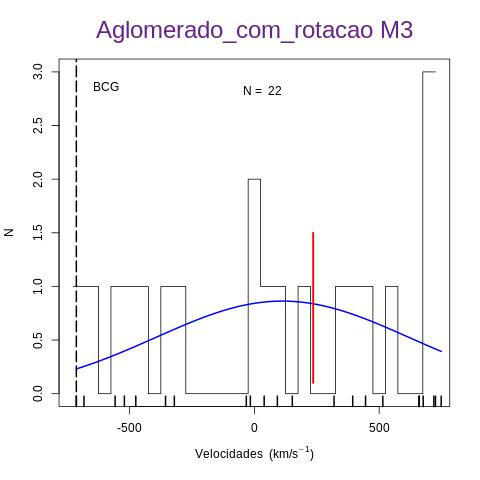
\includegraphics[scale=.23]{resultados/dist3}}
\subfloat{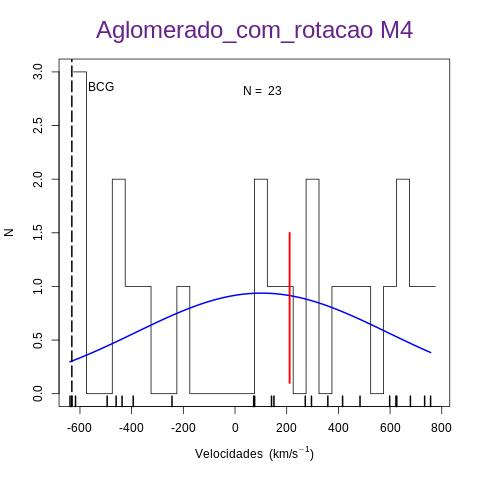
\includegraphics[scale=.23]{resultados/dist4}}\hfill
\subfloat{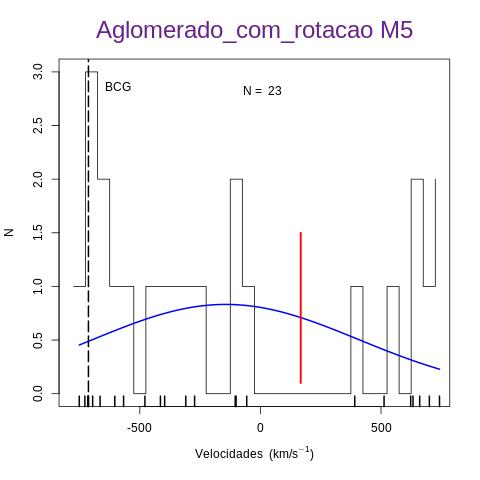
\includegraphics[scale=.23]{resultados/dist5}}
\subfloat{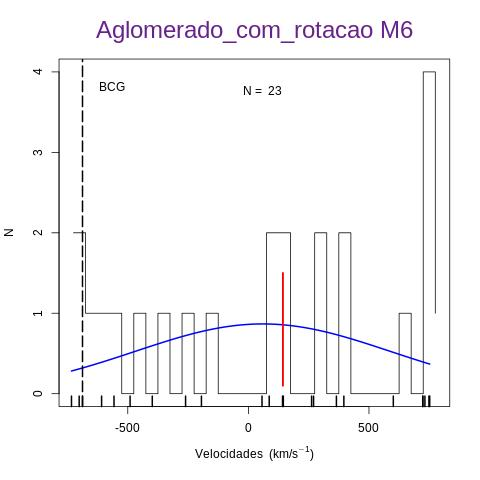
\includegraphics[scale=.23]{resultados/dist6}}
\subfloat{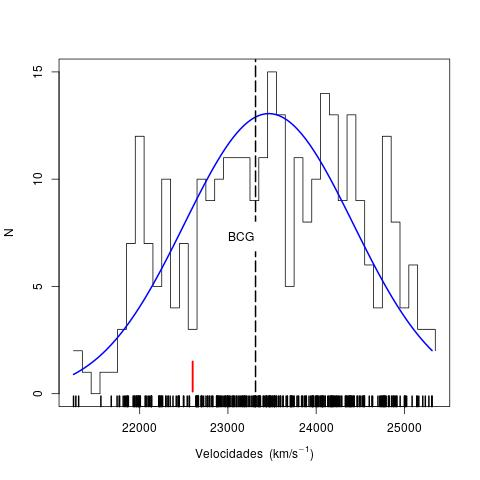
\includegraphics[scale=.23]{resultados/dist7}}
\subfloat{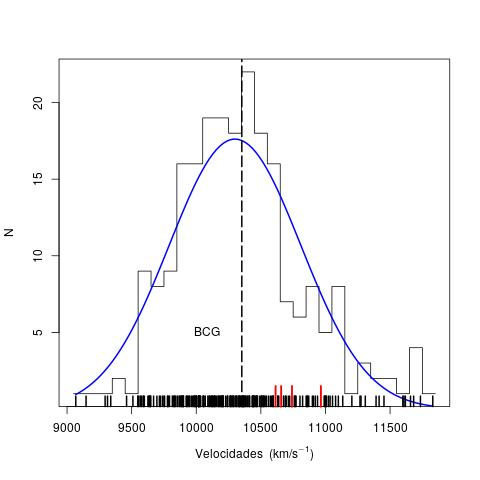
\includegraphics[scale=.23]{resultados/dist8}}\hfill
\subfloat{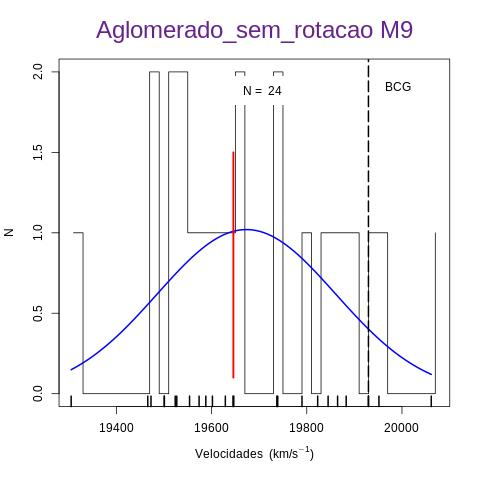
\includegraphics[scale=.23]{resultados/dist9}}
\subfloat{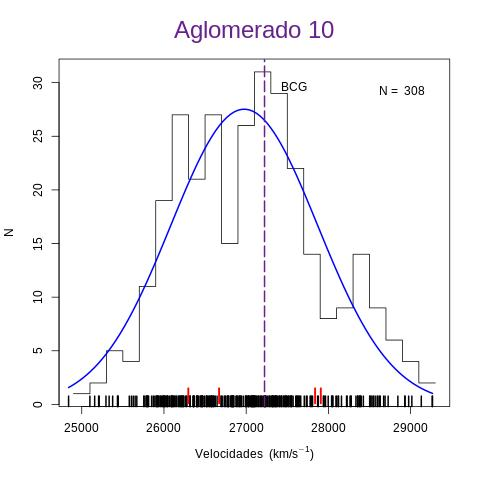
\includegraphics[scale=.23]{resultados/dist10}}
\subfloat{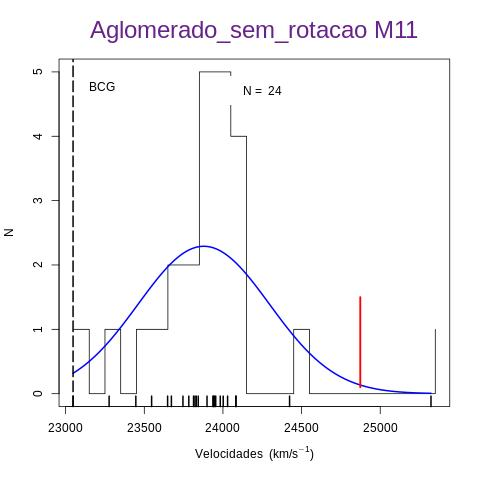
\includegraphics[scale=.23]{resultados/dist11}}
\subfloat{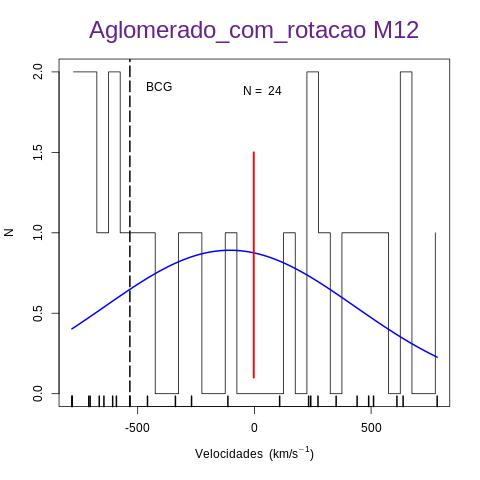
\includegraphics[scale=.23]{resultados/dist12}}\hfill
\subfloat{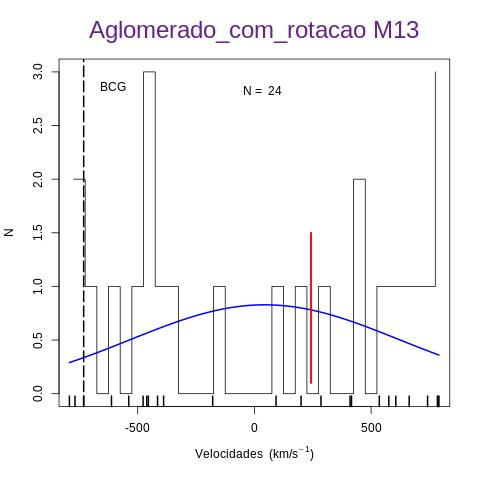
\includegraphics[scale=.23]{resultados/dist13}}
\subfloat{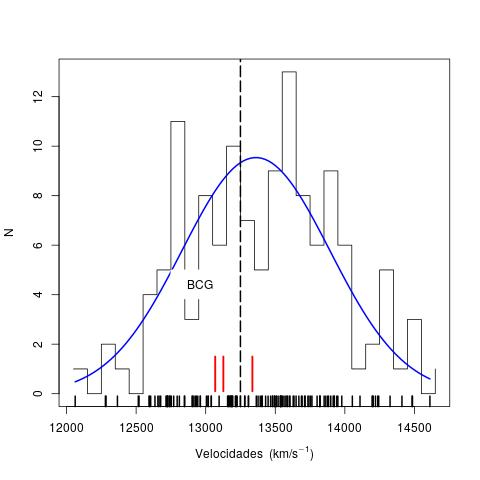
\includegraphics[scale=.23]{resultados/dist14}}
\subfloat{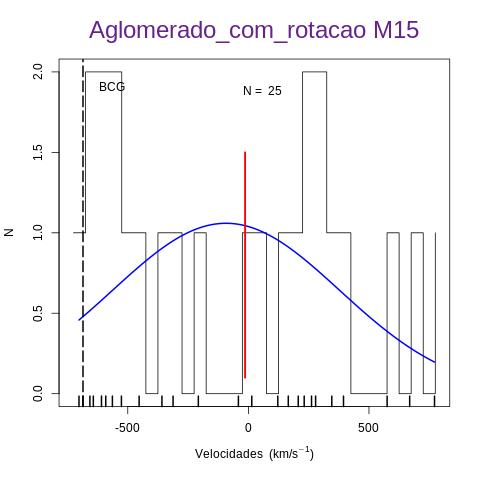
\includegraphics[scale=.23]{resultados/dist15}}
\subfloat{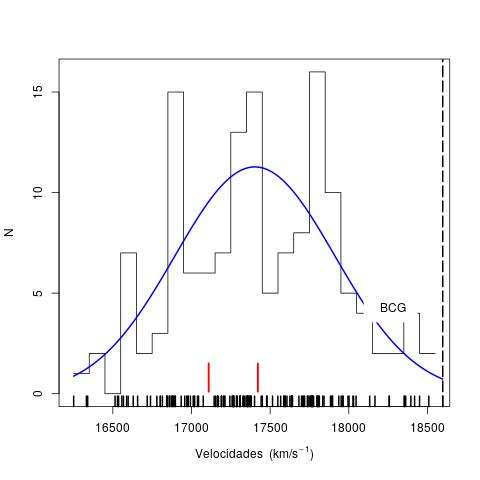
\includegraphics[scale=.23]{resultados/dist16}}\hfill
\subfloat{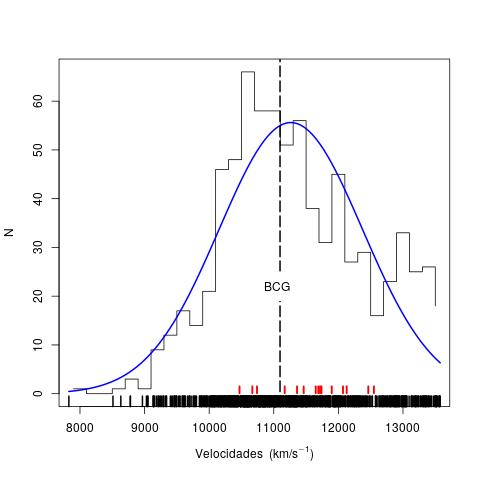
\includegraphics[scale=.23]{resultados/dist17}}
\subfloat{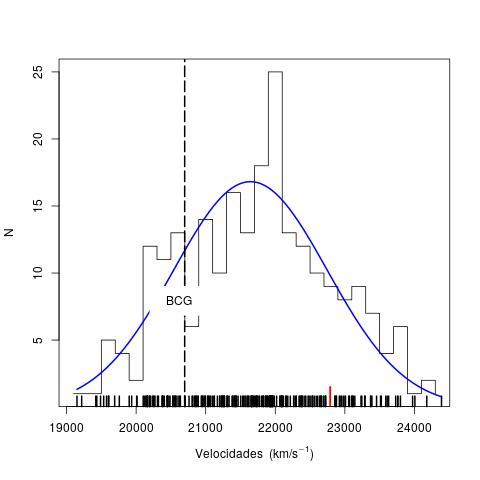
\includegraphics[scale=.23]{resultados/dist18}}
\subfloat{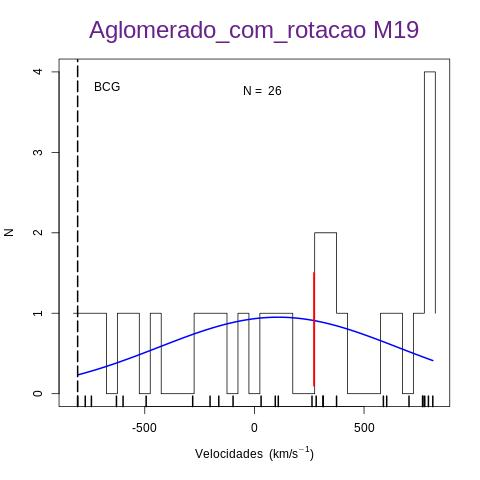
\includegraphics[scale=.23]{resultados/dist19}}
\subfloat{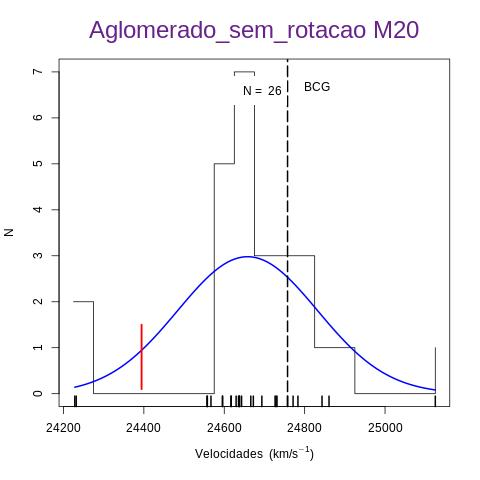
\includegraphics[scale=.23]{resultados/dist20}}
\caption{Histograma Distribuição de Velocidade e Análise de Gaps.}
\label{fig:fig4}%
\end{figure}


\begin{figure}[H] %h or !htbp
\vspace{-2pt}
\begin{center}
\subfloat{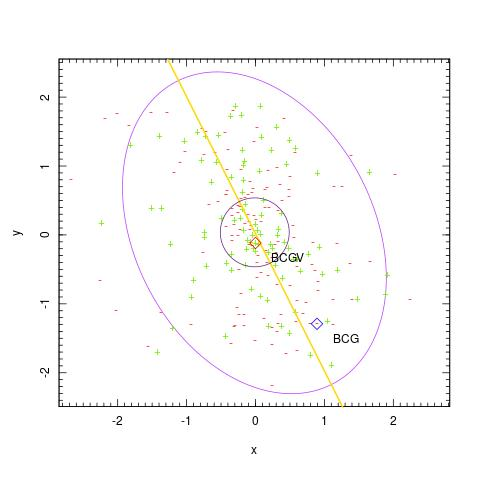
\includegraphics[scale=.23]{resultados/eixo1}}
\subfloat{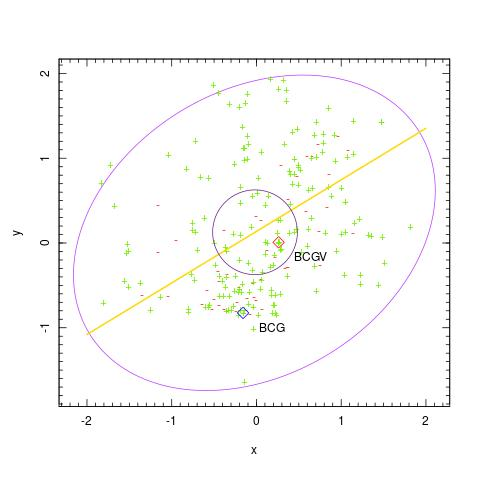
\includegraphics[scale=.23]{resultados/eixo2}}
\subfloat{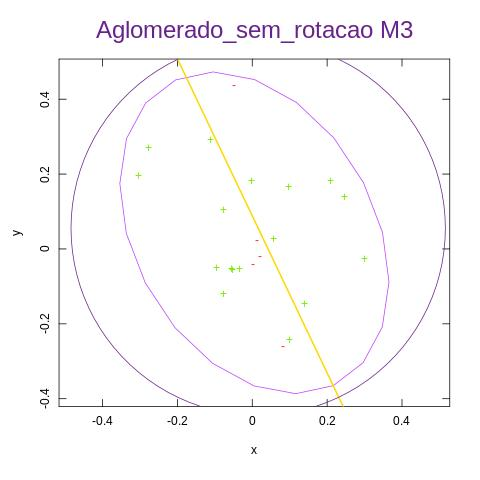
\includegraphics[scale=.23]{resultados/eixo3}}
\subfloat{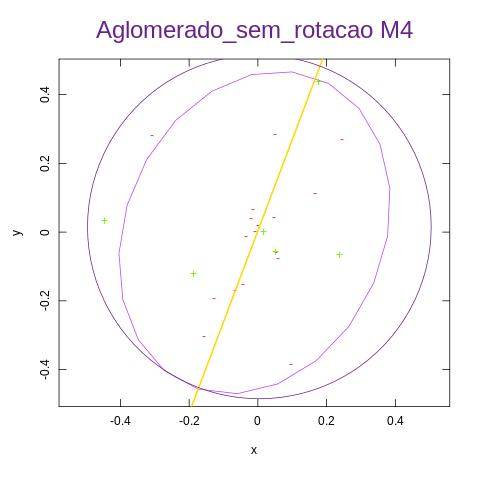
\includegraphics[scale=.23]{resultados/eixo4}}\hfill
\subfloat{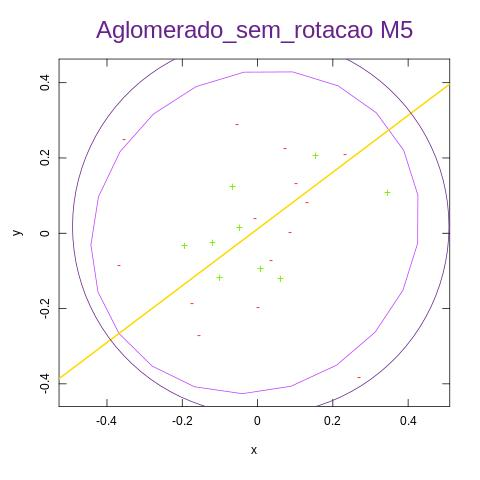
\includegraphics[scale=.23 ]{resultados/eixo5}}
\subfloat{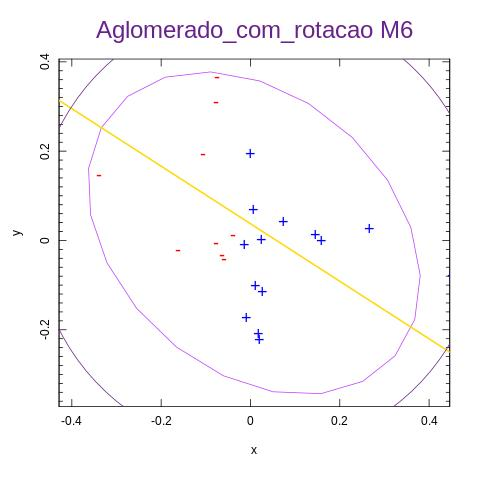
\includegraphics[scale=.23 ]{resultados/eixo6}}
\subfloat{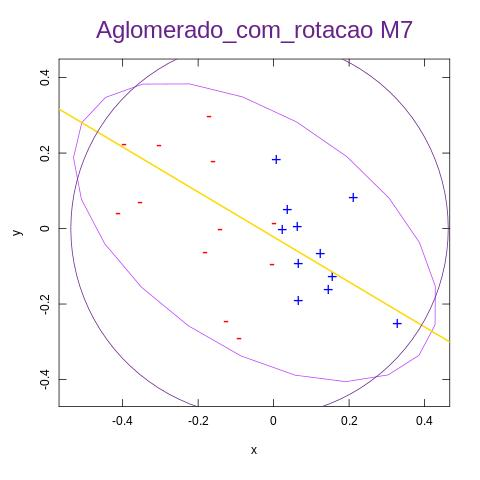
\includegraphics[scale=.23 ]{resultados/eixo7}}
\subfloat{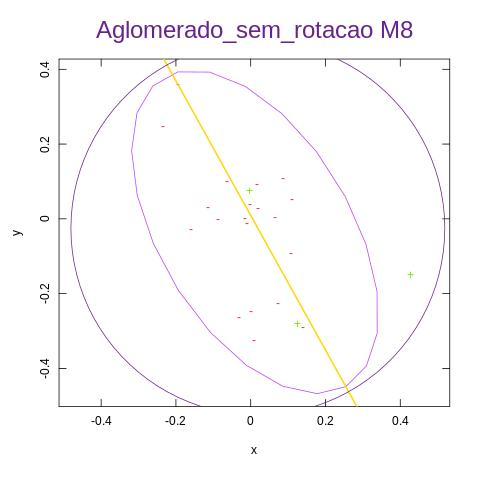
\includegraphics[scale=.23 ]{resultados/eixo8}}\hfill
\subfloat{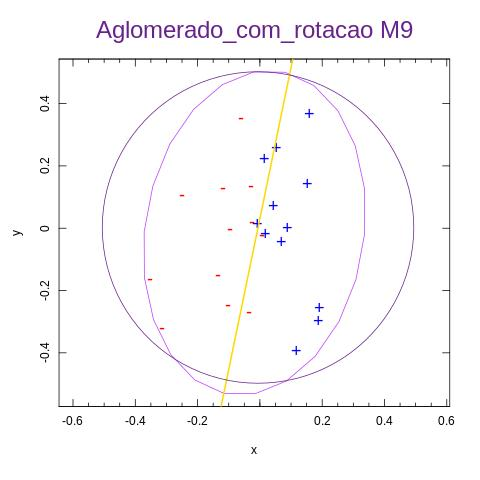
\includegraphics[scale=.23 ]{resultados/eixo9}}
\subfloat{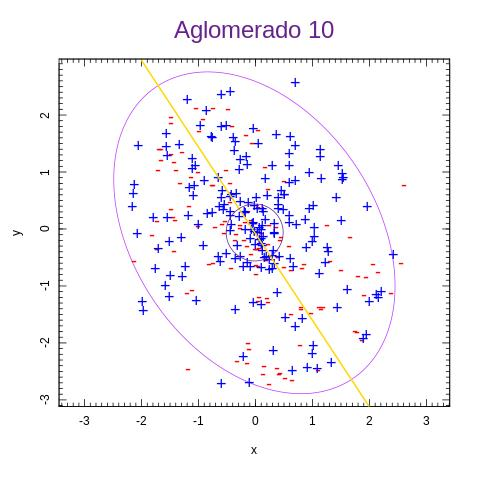
\includegraphics[scale=.23 ]{resultados/eixo10}}
\subfloat{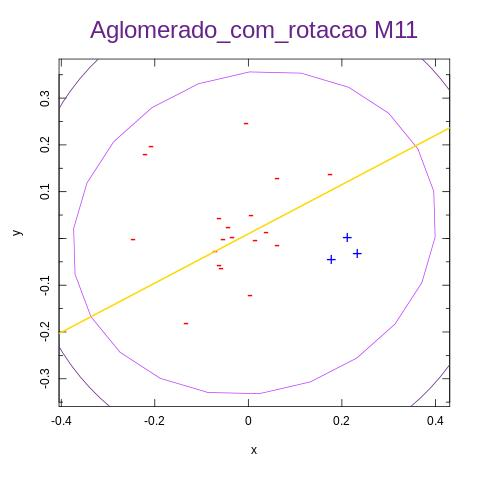
\includegraphics[scale=.23 ]{resultados/eixo11}}
\subfloat{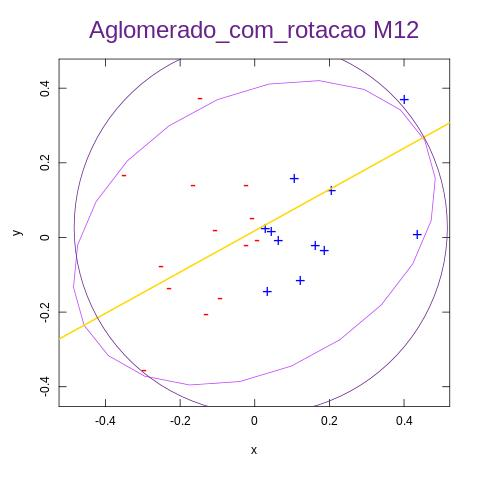
\includegraphics[scale=.23 ]{resultados/eixo12}}\hfill
\subfloat{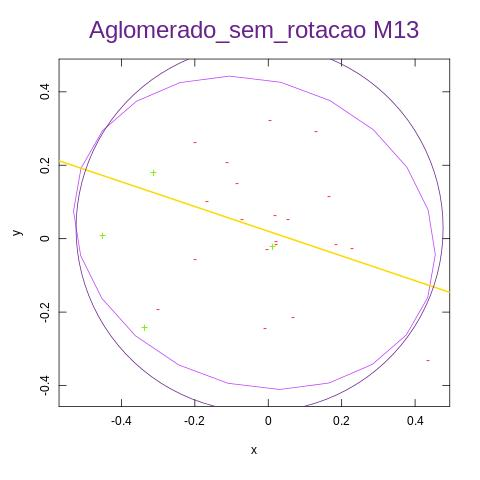
\includegraphics[scale=.23 ]{resultados/eixo13}}
\subfloat{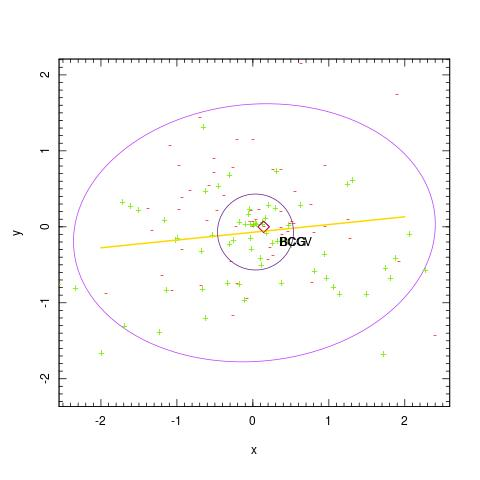
\includegraphics[scale=.23 ]{resultados/eixo14}}
\subfloat{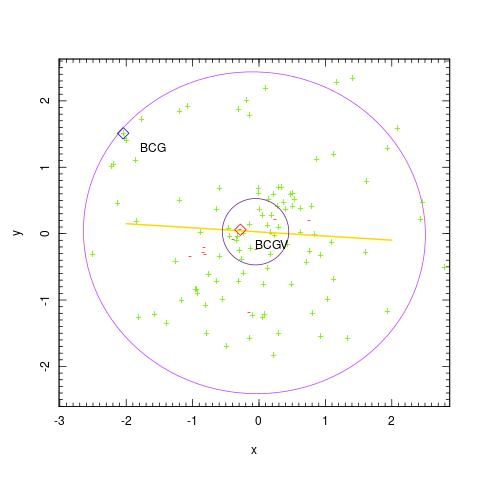
\includegraphics[scale=.23 ]{resultados/eixo15}}
\subfloat{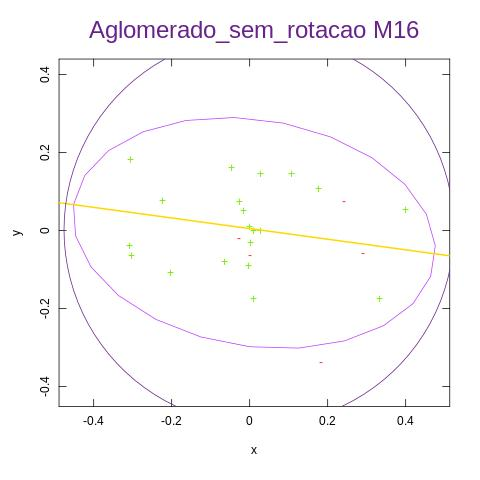
\includegraphics[scale=.23 ]{resultados/eixo16}}\hfill
\subfloat{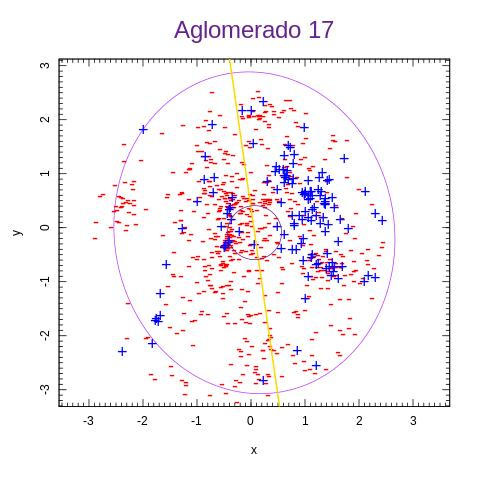
\includegraphics[scale=.23 ]{resultados/eixo17}}
\subfloat{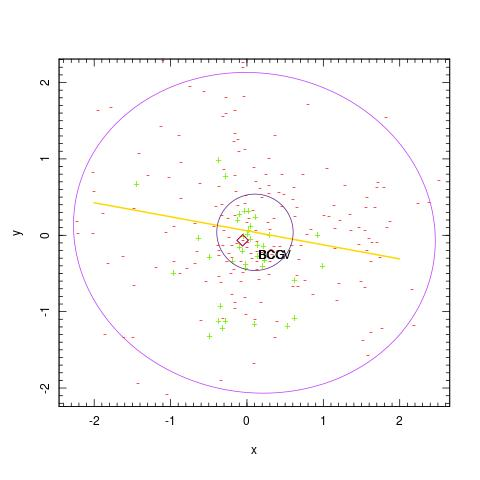
\includegraphics[scale=.23 ]{resultados/eixo18}}
\subfloat{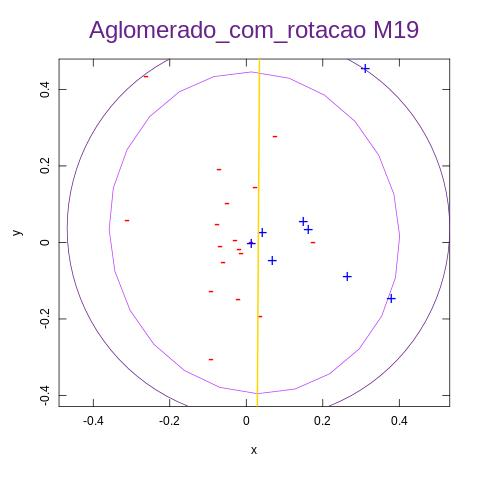
\includegraphics[scale=.23 ]{resultados/eixo19}}
\subfloat{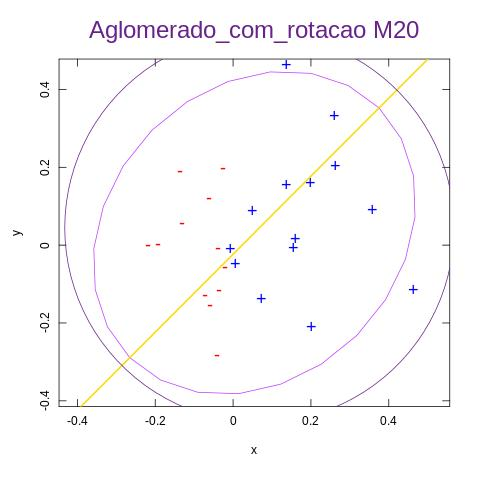
\includegraphics[scale=.23 ]{resultados/eixo20}}
\caption{Ajuste da elipse e eixo principal da distribuição projetada no plano do céu.}
\label{fig5}%
\end{center}
\end{figure}

\begin{table}[H]
\caption{Teste Cramer e Hotelling em todos os pontos.}
\vspace{12pt}
\centering{}
\resizebox{.8\textwidth}{!}{
\begin{tabular*}{\textwidth}{@{\extracolsep{\fill}}ccc}     
\hline
\textbf{Aglomerado} & \textbf{Teste de Cramer \textit{p-value}} & \textbf{Teste de Hotelling \textit{p-value}} \\
\hline
 01 & 0.5064 & 0.6160 \\  
%\hline
 02 &{\color{red}  0.0059} & {\color{red} 0.0078}\\ 
%\hline
 03 & 0.3376  & 0.5612   \\ 
%\hline
 04 & {\color{red}0.0009} & {\color{red}$<$0.0001} \\ 
%\hline
 05 &  0.1018 &  {\color{red}0.0723} \\ 
%\hline
 06 &  0.2357 &   0.8041 \\ 
%\hline
 07 & 0.0519 &   0.6347 \\ 
%\hline
 08 & {\color{red}0.0069}  &  0.0807 \\ 
%\hline
 09 & {\color{red}0.0279} &  {\color{red}0.0373}  \\ 
%\hline
 10 & {\color{red}0.0009} & {\color{red}0.0258}   \\ 
%\hline
 11 &  {\color{red}0.0049} & 0.9006  \\ 
%\hline
 12 & {\color{red}$<$0.0001} & {\color{red}$<$0.0001}\\ 
%\hline
 13 &  0.1148  &   0.1516   \\ 
%\hline
 14 & {\color{red}0.0289} & {\color{red}0.0054}  \\ 
%\hline
 15 & 0.1148 & 0.5745 \\ 
%\hline
 16 & 0.0629 &  0.5182 \\ 
%\hline
 17 & $<$0.0001 &  $<$0.0001\\ 
%\hline
 18 & {\color{red}$<$0.0001} &  {\color{red}0.0075}\\ 
%\hline
 19 & 0.0939 &   0.4063\\ 
%\hline
 20 &  0.1018 & 0.9038 \\
\hline
\label{table1}
\end{tabular*}
}
\end{table}

\begin{table}[H]
\caption{Teste Cramér e Hotelling pontos acima do eixo.}
\vspace{12pt}
\centering{}
\resizebox{.8\textwidth}{!}{
\begin{tabular*}{\textwidth}{@{\extracolsep{\fill}}ccc}     
\hline
\textbf{Aglomerado} & \textbf{Teste de Cramer \textit{p-value}} & \textbf{Teste de Hotelling \textit{p-value}} \\
\hline
 01 & 0.7772 & 0.8718 \\  
%\hline
 02 &  0.0959 &  {\color{red}0.0069} \\ 
%\hline
 03 & 0.6623 & 0.2025  \\ 
%\hline
 04 & {\color{red}0.0009} & {\color{red}$<$0.0001} \\ 
%\hline
 05 &  {\color{red}0.0319} & {\color{red}0.0483}  \\ 
%\hline
 06 &  0.4575 &   0.2650 \\ 
%\hline
 07 & 0.5894&  0.5880\\ 
%\hline
 08 &  {\color{red}0.0049}  &  0.4446 \\ 
%\hline
 09 &  {\color{red}0.0389}  &  0.2302 \\ 
%\hline
 10 & {\color{red}0.0029} & {\color{red}0.0067 } \\ 
%\hline
 11 &  0.3386 &  {\color{red}0.0031} \\ 
%\hline
 12 &{\color{red} $<$0.0001 }& {\color{red}$<$0.0001}\\ 
%\hline
 13 &  0.1518  &   0.6982  \\ 
%\hline
 14 &  0.4795 & 0.0054  \\ 
%\hline
 15 & 0.3406  & 0.5745 \\ 
%\hline
 16 & {\color{red}0.0059} &  0.5182 \\ 
%\hline
 17 & {\color{red}$<$0.0001} & {\color{red}$<$0.0001} \\ 
%\hline
 18 & {\color{red}0.0169} &  {\color{red}0.0075}\\ 
%\hline
 19 & 0.2817 &   0.4063\\ 
%\hline
 20 &  0.0699 & 0.3173 \\
\hline
\label{table2}
\end{tabular*}
}
\end{table}

\begin{table}[H]
\caption{Teste Cramer e Hotelling pontos abaixo do eixo.}
\vspace{12pt}
\centering{}
\resizebox{.8\textwidth}{!}{
\begin{tabular*}{\textwidth}{@{\extracolsep{\fill}}ccc}     
\hline
\textbf{Aglomerado} & \textbf{Teste de Cramer \textit{p-value}} & \textbf{Teste de Hotelling \textit{p-value}} \\
\hline
 01 & 0.3836 & 0.7469 \\  
%\hline
 02 &{\color{red} 0.0299} &  0.0916 \\ 
%\hline
 03 & 0.0759  & 0.1299  \\ 
%\hline
 04 & {\color{red}$<$0.0001} & {\color{red}$<$0.0001} \\ 
%\hline
 05 &  0.1018 & {\color{red}0.0483}  \\ 
%\hline
 06 &  0.2357 &   0.2650 \\ 
%\hline
 07 & 0.0519 &  0.5880\\ 
%\hline
 08 & {\color{red}0.0069}  &  0.4446 \\ 
%\hline
 09 & {\color{red}0.0279} &  0.2302 \\ 
%\hline
 10 & {\color{red}0.0009} & {\color{red}0.0067}  \\ 
%\hline
 11 &  {\color{red}0.0049} &  {\color{red}0.0031} \\ 
%\hline
 12 & {\color{red}$<$0.0001} & {\color{red}$<$0.0001}\\ 
%\hline
 13 &  0.1148  &   0.6982  \\ 
%\hline
 14 & {\color{red}0.0289} & {\color{red}0.0054}  \\ 
%\hline
 15 & 0.1148 & 0.5745 \\ 
%\hline
 16 & 0.0629 &  0.5182 \\ 
%\hline
 17 & {\color{red}$<$0.0001} &  {\color{red}$<$0.0001}\\ 
%\hline
 18 & {\color{red}$<$0.0001} &  {\color{red}0.0075}\\ 
%\hline
 19 & 0.0939 &   0.4063\\ 
%\hline
 20 &  0.1018 & 0.9038 \\
\hline
\label{table3}
\end{tabular*}
}
\end{table}


\begin{figure}[H] %h or !htbp
\vspace{-2pt}
\begin{center}
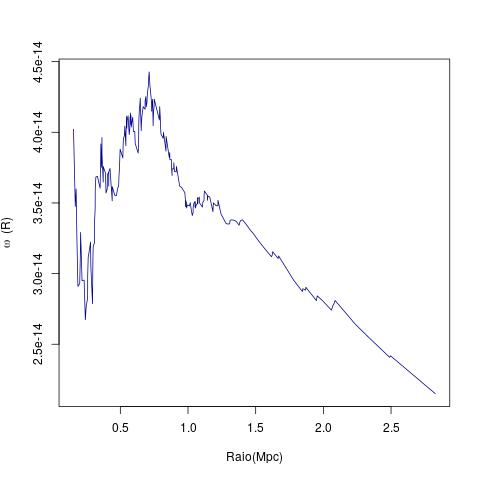
\includegraphics[scale=.3]{resultados/perfil2}%
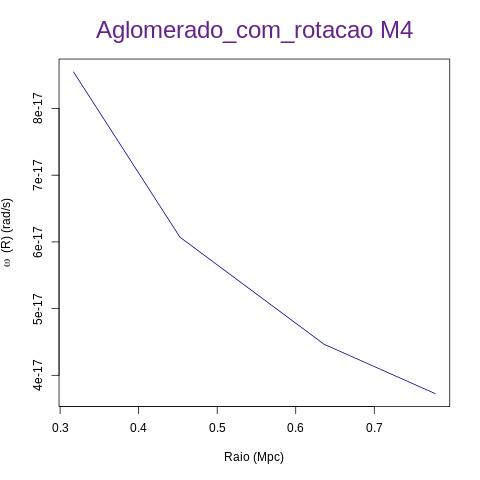
\includegraphics[scale=.3]{resultados/perfil4}
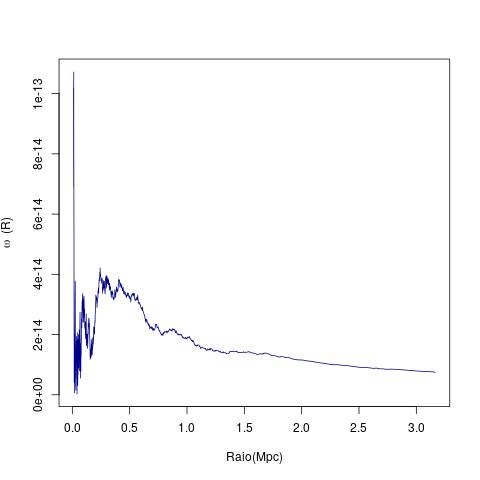
\includegraphics[scale=.3]{resultados/perfil5}\hfill
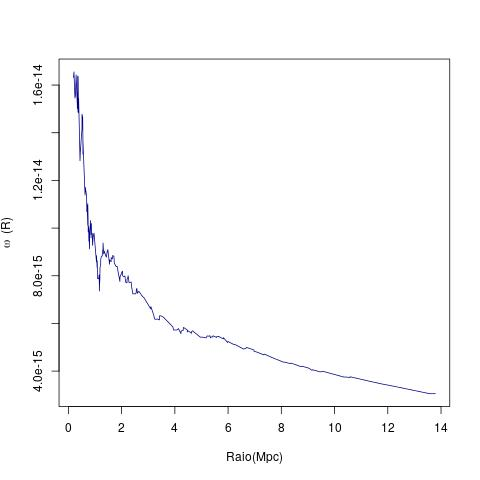
\includegraphics[scale=.3]{resultados/perfil8}
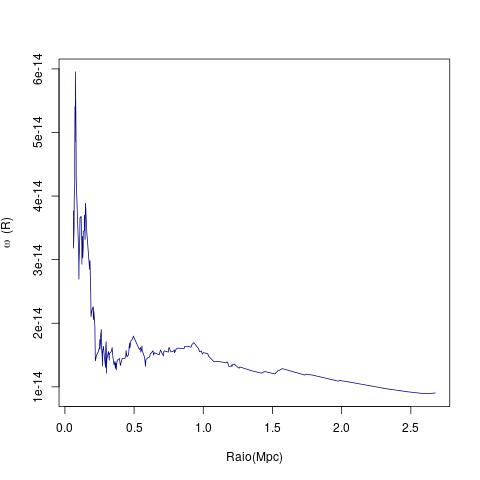
\includegraphics[scale=.3]{resultados/perfil9}%
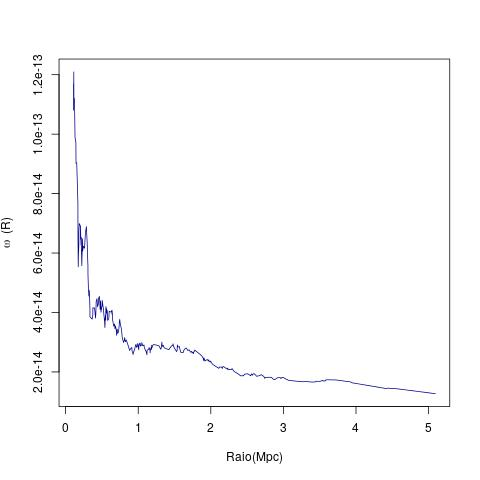
\includegraphics[scale=.3]{resultados/perfil10}\hfill
\includegraphics[scale=.3]{resultados/perfil11}%
\includegraphics[scale=.3]{resultados/perfil12}
\includegraphics[scale=.3]{resultados/perfil14}\hfill
\includegraphics[scale=.3]{resultados/perfil16}
\includegraphics[scale=.3]{resultados/perfil17}%
\includegraphics[scale=.3]{resultados/perfil18}%
\caption{Perfil da velocidade de rotação.}
\label{fig6}%
\end{center}
\end{figure}

\section{Conclusões e Perspectivas}

Apresentamos um método de detecção de rotação em aglomerados de galáxias desenvolvido em R.
Nosso objetivo foi investigar um dos aspectos menos estudados a respeito de aglomerados, que é a possibilidade de que eles tenham algum grau de rotação. Não levar em consideração a rotação de aglomerados pode gerar um erro nas suas estimativas de massa. O entendimento, controle e redução deste tipo de erro são de grande importância para a astrofísica extragaláctica. Nossos resultados indicam que
12 entre os 20 aglomerados de galáxias podem ser sistemas girantes.

Entre os próximos passos em nosso trabalho, pretendemos repetir o cálculo usando a mediana da distribuição, como no método de
Tovmassian (2015), e a definição de substruturas, quando existirem, para a divisão de aglomerados, ao invés do uso do {\it gap} principal. Além disso, faremos uma comparação de nosso método com aquele de Hwang \& Lee (2007).

O método de Hwang \& Lee utiliza a relação sinoidal para o cálculo do ângulo do eixo de rotação $\theta_o$ e a velocidade de rotação $v_{rot}$, definida na equação:

\begin{equation}
v_p(v_{rot}, \theta) = v_{sys} + v_{rot} * sin(\theta - \theta_o)
\label{eq:eq11}
\end{equation}

\noindent em que $v_p$ é a velocidade radial de cada galáxia em relação a rotação do aglomerado, $v_{sys}$ é a velocidade de cada galáxia do aglomerado e $\theta$ é o ângulo projetado de cada galáxia no plano do céu, no sentido Norte a Leste.  

Para determinação de valores mais adequados para $\theta$ e $v_{rot}$ utiliza-se o procedimento do $\chi^2$, representado na equação \ref{eq:eq12}, assumindo que o modelo senoidal represente bem os dados de velocidade.

\begin{equation}
\chi^2 (v_{rot}, \theta_o) = \sum_i \frac{({v_{pi} - v_{vlos,i})}^2}{\sigma^{2}_i}.
\label{eq:eq12}
\end{equation}

\noindent onde $v_{los,i}$ é a velocidade de linha de visão de cada galáxia e $\sigma_i$ é a medida de erro.

Além da implementação do método de Hwang \& Lee (20017), 
faz parte ainda de nossos objetivos aplicar nosso programa a um conjunto maior de dados
e ter um resultado estatisticamente mais robusto acerca da fração de aglomerados
que apresentam rotação no Universo Local. Para isto, já selecionamos uma amostra
com aproximadamente 500 aglomerados do SDSS, definida originalmente por Nichols et al. (2005)
com dados do SDSS-DR2 e redefinida aqui com dados do SDSS-DR12. Será a maior amostra submetida
à análise de efeitos de rotação.


\newpage
% ------------------------------------------------------------------------
\begin{thebibliography}{99}
\fontsize{11}{0}\selectfont
\bibitem[Chluba \& Mannheim, 2002]{chluba2002}
Chluba, J.; Mannheim,. Kinetic Sunyaev-Zeldovich effect from galaxy cluster rotation. MNRAS, v. 396, p. 419 -
427, Agosto 2002.

\bibitem[Beers et~al., 1990]{Beers1990}
Beers, T. C., Flynn K., Gebhardt K., 1990, AJ, 100, 32. 

\bibitem[de Oliveira et~al., 2004]{deOliveira2004}
de Oliveira, F.; Viegas, S. M. M. Descobrindo o Universo. São Paulo: Edusp, v. 56, 2004.

\bibitem[Fang et~al, 2008]{Fang2008}
Fang, T.; Humphrey, P. J.; Buote, D. A. Rotation and Turbulence of the Hot ICM in Galaxy Clusters. MNRAS,
v. 691, p. 1648-1659, Agosto 2008.

\bibitem[Friaça et~al, 2008]{Friaca2008}
Friaça, A. C. S. et al. Astronomia: Uma Visão Geral do Universo. 2a. ed. São Paulo: EDUSP, v. 28, 2008.

\bibitem[Hamden et~al, 2010]{Hamden2010}
Hamden, E. T. et al. Measuring Transverse Motions for Nearby Galaxy Clusters. MNRAS, Maio 2010.

\bibitem[Hwang \& Lee, 2007]{Hwang2007}
HWANG, Ho Seong; LEE, Myung Gyoon. Searching for rotating galaxy clusters in SDSS and 2dFGRS. {The Astrophysical Journal}, v. 662, n. 1, p. 236, 2007.

\bibitem[Kalinkov et~al, 2005]{Kalinkov2005}
Kalinkov, M. et al. Rotation of the cluster of galaxies A2107. MNRAS, v. 359 , p. 1491-1497, Maio 2005.

\bibitem[Manolopoulou et~al., 2008]{Manolopoulou2016}
Manolopoulou, M.; Plionis, M. Galaxy cluster's rotation. MNRAS, v. 465 , p. 2616-2633, Abril 2016.

\bibitem[Nascimento, 2012]{Nascimento2012}
Nascimento, R. S. Estudo da dinâmica de pares de aglomerados de galáxias. Dissertação (Programa de Pós-
graduação em Física) - UESC. Ilhéus, p. 91. 2012.

\bibitem[Ribeiro et~al, 2011]{Ribeiro2011}
Ribeiro A. L. B., Lopes P. A. A., Trevisan M., 2011, MNRAS, 413, L81.

\bibitem[Rembold, 2011]{Rembold2011}
Rembold, B. Tópicos especiais em física: Astronomia. Ilhéus: UAB /UESC, v. 4, 2011. 384 p.

\bibitem[Sampaio, 2013]{Sampaio2013}
Sampaio, F. S. Estudo da Distribuição de velocidades em aglomerados de galáxias - Testes de Não Rejeitaidade e
metanálise de Fisher. Dissertação (Programa de Pós-Graduação em Física) - UESC. Ilhéus, p. 51. 2013.

\bibitem[Tovmassian, 2015]{Tovmassian2015}
Tovmassian, H. M. The rotation of Galaxy Clusters. Astrophysics, v. 58, p. 353-363, Setembro 2015.

\bibitem[Velásquez, 2007]{Velasquez2017}
Velásquez, C. A. M. Estimativa de Parâmetros Cosmológicos usando Aglomerados de Galáxias. Dissertação
(Programa de Pós-Graduação em Astronomia) - UFRJ. Rio de Janeiro, p. 74. 2007.

\bibitem[Yahil et~al., 1997]{Yahil1997}
Yahil, A \& Vidal, N. V The Velocity Distribution Of Galaxies In Clusters Ap. J. N 214, 347-350, 1997.
\end{thebibliography}

\newpage

\section{APÊNDICE}

\subsection{Testes de Hipótese}
A análise estatística objetiva, especialmente, fazer inferência sobre uma população a partir da observação de uma amostra. Os testes de hipótese representam uma forma de inferência estatística. A hipótese é uma afirmação sobre parâmetros populacionais que devem ser analisadas para verificar sua veracidade. É importante ressaltar que a verdade ou não nunca pode ser determinada, a menos que toda a população seja observada, situação impraticável na maioria das vezes, justificado pelo uso do teste estatístico. 

A princípio é necessário estabelecer como verdadeira a \textbf{hipótese nula}, denotada por \textbf{$H_0$}. Já a \textbf{hipótese alternativa} (\textbf{$H_1$}), contrapõe a hipótese nula, ou seja, $H_0$ deverá ser rejeitada. É necessário estabelecer um critério auxiliar para decidir a rejeição ou não de H0 para um teste estatístico. Esse valor, determinado pelo pesquisador antes da análise de dados ou até mesmo na coleta de dados, cenário ideal, é denominado \textbf{nível alfa ($\alpha$) ou nível de significância}. Comumente é utilizado como critério de rejeição uma probabilidade de 5%. De acordo com Cramer e Howitt (2004),

\begin{quote}
O nível em que a hipótese nula é rejeitada é geralmente definido como 5 ou menos vezes fora de 100. Isso significa que tal diferença ou relacionamento é provável que ocorra por acaso 5 ou menos vezes de 100. Este nível é geralmente descrito como proporção 0.05 e às vezes como a porcentagem 5\%. O nível de probabilidade de 0.05 foi historicamente uma escolha arbitrária, mas tem sido aceitável como uma escolha razoável na maioria das circunstâncias. Se houver um motivo para variar este nível, é aceitável fazer então. Então, em circunstâncias em que pode haver consequências adversas muito graves se a decisão errada foi feita sobre a hipótese, então o nível de significância poderia ser mais rigoroso em, digamos, 1\% (Cramer and Howitt, 2004: 151).
\end{quote}

Na realização de testes de hipóteses é possível que erros sejam cometidos, como mostrado na tabela 1. \textbf{Erro do tipo I}, denotado por \textbf{erro $alpha$}, a rejeição de $H_0$ quando ela é verdadeira. Contrapondo, a não-rejeição de $H_0$ quando esta é falsa é denominada \textbf{erro do tipo II} e representado por \textbf{$\beta$}.  Esse tipo de teste permite concluir se deve aceitar ou rejeitar a hipótese nula, porém não é possível quantificar o quão provável é o resultado de ocorrer ao acaso. Apoiado por isto, é definido a potência de um teste estatístico $1-\beta$ como a probabilidade de rejeitar H0 quando de fato é falsa. Claramente, o teste ideal é aquele em que os valores de $\alpha$ e $\beta$ são mínimos. Porém, o valor de $\alpha$ é inversamente relacionado com o valor de $\beta$, sendo impossível minimizá-los simultaneamente. Geralmente, é fixado o nível de significância $\alpha$ e escolhido a região de rejeição que minimiza $\beta$, ou seja, que maximize a potência do teste. 

% TABLE EXAMPLE
\begin{table}[H] % !htbp 
\caption{Tipos de erros em testes de hipótese}
\vspace{12pt}
\centering{}
\resizebox{.8\textwidth}{!}{
\begin{tabular*}{\textwidth}{@{\extracolsep{\fill}}ccc}     
\hline
\multirow{3}{*}{\textbf{Decisão estatística}} 
      & \multirow{1}{*}{\textbf{Natureza (estado verdadeiro ou desconhecido)}}\\
      & {\boldmath$H_0$} \textbf{verdadeira} & {\boldmath $H_0$} \textbf{falsa} \\
\hline
\textbf{Aceitar \boldmath $H_0$}  & acerto &  Erro tipo II ($\beta$) \tabularnewline
\hline
\textbf{Rejeitar \boldmath $H_0$}  & Erro tipo I ($\alpha$) &  acerto \tabularnewline
\hline
\label{table0}
\end{tabular*}
}
\end{table}

O menor nível de significância pode ser definido utilizando o \textbf{valor-p} ou \textit{\textbf{“p-value”}}. No teste de hipótese esse valor é comparado ao nível de significância $\alpha$ determinado no início objetivando a tomada de decisão de aceitar ou rejeitar $H_0$. Se o valor-p calculado do teste for igual ou maior que $\alpha$, a $H_0$ é aceita. Ou seja, a hipótese nula é consistente com os resultados da amostra. Porém, se o valor-p for menor que $\alpha$, a hipótese nula é rejeitada, a hipótese alternativa, nesse caso, é então aceita como verdadeira. 

\subsection{Teste de Comparação entre duas amostras}
Uma variável aleatória, seja idade de um grupo de pessoas ou ocorrência de um determinado desfecho, pode admitir uma distribuição de frequências da população, contendo diversas formas encontradas na literatura estatística. O intuito desses modelos é caracterizar o comportamento de um determinado evento em função da frequência de sua ocorrência. Se as variáveis forem contínuas, o evento será um intervalo de valores. Portanto, as distribuições de frequências são efetivamente distribuições de probabilidade, em que para um evento teremos associado uma probabilidade de ocorrência.

A inspeção visual pode ser utilizada para avaliação da comparação entre duas amostras. A distribuição de frequência, como exemplo um histograma, relaciona valores observados à sua frequência e pode além de pressupor uma distribuição Não Rejeita, identifica insights sobre lacunas nos dados e outliers. O histograma é composto por barras justapostas em que no eixo horizontal contém a variável de interesse dividida em classes e no eixo vertical a sua correspondente frequência. Para distribuições do tipo Não Rejeita ou Gaussiana, o histograma constitui formato de sino (Figura \ref{fig2}).

Entretanto, a simples constatação por meio de gráficos é subjetiva e não satisfatória, pois depende de uma interpretação visual além de não ser confiável no caso multivariado e especificamente nas situações de muitas variáveis. Desta forma, para inferir sobre a comparação entre duas amostras é necessário utilizar como complemento testes estatísticos (T1).  Como exemplo, podemos citar: o teste de aderência qui-quadrado; Kolmogorov-Smirnov; Lilliefors e Shapiro-Wilk. 

Estes testes possuem estatísticas de teste e critérios de decisão diferentes, porém compartilham da hipótese avaliada: a hipótese de nulidade ($H_0$) especifica que a variável aleatória adere à distribuição Não Rejeita, sem a necessidade de definir a média ou variância da distribuição. Já a hipótese alternativa ($H_1$), opõe a hipótese nula.

O resultado que interessa após executar um determinado teste é o seu valor-p ou nível descritivo do teste, referente à probabilidade de que a estatística do teste (como variável aleatória) tenha valor extremo em comparação ao valor observado (estatística) quando a hipótese nula é verdadeira. Sendo o valor-p menor que o nível de significância, logo a hipótese nula é rejeitada. Ou seja, o valor-p representa o menor nível de significância que pode assumir para então rejeitar a hipótese nula. Logo, há significância estatística quando o valor-p é menor que o nível de significância estabelecido.

\subsection{Testes Utilizados}

\vspace{0.5cm}
\textbf{\textit{Teste de Cramer.}} Em estatística, o teste de Cramér (conhecido também como phi de Cramer - $\varphi$c) é uma medida de associação entre duas variáveis nominais dado o intervalo de 0 a 1, indicando que um valor mais alto possui forte associação. Fundamentado no teste estatístico do qui-quadrado de Pearson, foi publicado em 1946 por Harald Cramér. A medida é definida como 

\begin{equation}
\ V = \sqrt{\frac{{\chi_{obt}}^2}{N.m}}
\label{eq:eq1}
\end{equation}
	
	onde $\chi^2$ é o valor obtido do teste estatístico
	
	N é o tamanho da amostra e 
    
    m = o menor de (r - 1) ou (c – 1), sendo r o número de linhas e c o número de colunas.

Para entender melhor a utilidade do teste de Cramer é fundamental compreender as formas como os testes estatísticos divergem das medidas de associação para variáveis categóricas. O teste qui-quadrado ($\chi^2$) fornece um teste estatístico de associação entre duas variáveis categóricas (nominais) de uma população única. Ele determina se a associação entre as variáveis é significativa, utilizando como hipótese nula ($H_0$) que as duas variáveis não são dependentes uma da outra e como hipótese alternativa ($H_1$) é que existe alguma associação entre duas variáveis.

O teste de Cramer é considerado um dos favoritos entre as medidas baseadas no qui-quadrado. Geralmente, quando o seu cálculo resulta no valor máximo 1 é que exista um forte relacionamento entre duas variáveis. No cálculo de Cramer é levado em consideração as dimensões da tabela, ou seja, diferentes dimensões podem ser comparadas significativamente.

\vspace{0.5cm}
\textbf{\textit{Teste de Hotelling.}} Um dos mais conhecidos testes de hipóteses multivariados foi proposto por Harold Hotelling em 1947, o teste de $T^2$, compara vetores de médias populacionais. Baseado na generalização da estatística \textit{t de Student}, foi o primeiro a levar em consideração a correlação das variáveis na formulação da estatística do teste.

Sendo \textbf{\textit{X}} um vetor aleatório com uma dada dimensão, \textbf{\textit{$\mu$}} o vetor de médias e \textbf{\textit{$\sigma$}} a matriz de covariância. Para \textbf{\textit{X}}, sendo uma distribuição Não Rejeita multivariada e com tamanho de amostra aleatória \textbf{\textit{n}}, a estatística de $T^2$ é dada por
\begin{equation}
\ T^2 = n(\overline{X} - \mu_0) \sum_{pxp}^{-1} {(\overline{X} - \mu_0)}
\label{eq:eq2}
\end{equation}

com

\begin{equation}
 H_0 : \mu = \mu_0 \\
 H_1 : \mu \neq \mu_0
\label{eq:eq3}
\end{equation}

A equação \ref{eq:eq2} tem distribuição qui-quadrado com \textit{p} graus de liberdade. Definindo um nível de significância $\alpha$, com $0 < \alpha < 1$, para valores de $T^2$  maiores ou iguais ao valor crítico ${\chi^2_{a,p,c}}$ dado por $P[{\chi_p}^2 \geq {\chi^2_{a,p,c}}]$,  a hipótese nula será rejeitada.   

Sendo a matriz desconhecida, a estatística de $T^2$ é dada por

\begin{equation}
T^2 = n(\overline{X} -\mu_0) S^{-1}(\overline{X} - \mu_0)
\label{eq:eq4}
\end{equation}

que sob a hipótese nula, tem uma distribuição proporcional a uma distribuição F, ou seja, o valor crítico do teste a um nível de significância $\alpha$, com $0 < \alpha < 1$, é

\begin{equation}
F_c = \frac{p(n-1)}{n-p} F_{1-\alpha, p, n - p}
\label{eq:eq5}
\end{equation}

onde $F_{1-\alpha, p, n - p}$ é a probabilidade acumulada igual a (1 - $\alpha$) da distribuição de F com p
n-p é igual a graus de liberdade.

Sendo S a matriz de covariâncias amostrais (\textit{pxp}), um estimado não viciado de $\sum_pxp$, dado por
\begin{equation}
S = S^2_1, S_{1,2} ... S^2_2 ... S_{2,p} : S^2_p 
\label{eq:eq6}
\end{equation}

em que os elementos da diagonal principal de S são as variâncias definidos por
\begin{equation}
S^2_j = \frac{1}{m-1} \sum_{k=1}^m (x_{jk} - \overline{X}_j),    j = 1, 2, ..., 3 
\label{eq:eq7}
\end{equation}

e os elementos fora da diagonal principal são as covariâncias conforme

\begin{equation}
S_{jh} = \frac{1}{m-1} \sum_{k=1}^m (x_{jk} - \overline{X}_j)(x_{hk} - \overline{X}_h) 
\label{eq:eq8}
\end{equation}

onde $x_{jk}$ e $x_{hk}$ representam os valores amostrais das variáveis $X_j$ e $X_h$.



\newpage
%For papers written in Portuguese or Spanish.

\begin{center}
  ON THE ROTATION OF GALAXY CLUSTERS
\end{center}

\def\abstractname{Abstract}

\begin{abstract}
  Clusters of galaxies are the largest structures in the observable universe and consist
of a few tens to thousands of galaxies linked by gravitational force. They have properties such
as mass and spatial correlation functions, as well as their own evolution, considered tools
that can restrict the current cosmological model. Consequently, the precise calculation of
cluster masses is of utmost importance. There are several approaches to cluster mass
calculation, including a method that uses the velocities of the members of the cluster galaxy
and assumes dynamic equilibrium. This method does not take into account the possible
rotation of clusters. The rotation of these systems is due to an initial angular impulse that
lasts since their formation or as a result of mergers or interactions with neighbors.
Disregarding the rotation of clusters can lead to an error in calculating their mass that
directly affects the cosmological constraints provided by the mass function. In this work we
propose a method to identify the rotational component of clusters. The rotation detection
method was implemented in R, a multiparadigm language, and applied to a sample of 20
clusters, twelve of which showed significant rotation signal.
\end{abstract}

\keywords{\em{Galaxy clusters, Rotation, Statistical tests}}

\end{document}

\end{document}
